\documentclass[unicode,pdfcover]{hquthesis}
\usepackage{longtable,booktabs}
\usepackage{supertabular}
\usepackage{algorithm}
\usepackage{algpseudocode}
\usepackage{graphicx}
\usepackage[unicode=false,bookmarks=true,bookmarksnumbered=true,bookmarksopen=false,
 breaklinks=false,pdfborder={0 0 1},backref=false,colorlinks=true]
 {hyperref}

%%%%以下包可根据需要插入，基本涵盖所需内容。
\usepackage{multirow}%画表格推荐先在Excel简单制表，然后复制到该网页{Create LaTeX tables online https://tablesgenerator.com/}自动生成tex代码再粘贴过来（按需进一步简单修改）。
%\usepackage{arydshln}
%\usepackage{amsmath}%公式推荐使用WinEdt 10.3自带的IDE插入，公式外的特殊字符请使用$$ 括起来。
%\usepackage[算法]{algorithm}%算法二字可中文显示“算法”
%\usepackage{algorithmic}
\usepackage{lscape}%横放图表时用到
%\usepackage{longtable}%跨页表格用到

%模拟封面
\title{面向癌症基因数据集的混合协同集成聚类}
\author{李毅}
\authoren{Li Yi}
\supervisor{施一帆\ 副教授} 
\institute{华侨大学工学院}
\instituteen{College of Engineering, Huaqiao University}
\date{2026年4月}
\titleEN{Hybrid Collaborative Ensemble Clustering for Cancer Gene Expression Data}
\grade{2026}
\studentid{2295141020} %%%学号
\major{数据科学与大数据技术专业}
\majoren{Data Science and Big Data Technology}


\hypersetup{
	pdftitle={面向癌症基因数据集的混合协同集成聚类},
	pdfauthor={李毅},
	pdfsubject={华侨大学学位论文},
	linkcolor=black, anchorcolor=black, citecolor=black,
	filecolor=black, menucolor=black, urlcolor=black
}

\begin{document}
\maketitle

\frontmatter

\begin{abstractCN}
人工智能对癌症基因表达数据的分析很有用。在无监督情况下，集成聚类揭示了基因谱中固有的聚类结构，有助于医学和医疗保健研究的进步。然而，在处理癌症基因数据时，现有的集成聚类方法存在一些局限性：1)噪声特征影响聚类解的生成；2)聚类解的集成忽略了特征子空间；3)统一划分矩阵缺乏优化。在本文中，我们提出了一个用于癌症基因表达数据（HCEC）的混合协作集成聚类框架。首先，HCEC采用多种核化PCA方案提取压缩特征子空间，生成多种聚类方案，减少噪声干扰，从杂交的角度分析基因谱；然后，设计了一种新的共识广泛学习网络，该网络将多个特征子空间和聚类结构信息协同使用，以驱动更好的共识解决方案。通过参数分析、对比实验和消融研究，HCEC的有效性已经在多个真实世界的癌症基因表达数据集上得到了全面的证明。


\end{abstractCN}
\keywordsCN{集成聚类\kwsep 宽度学习系统\kwsep 癌症基因表达\kwsep 核主成分分析\kwsep 医疗人工智能}

\begin{abstractEN}
Artificial intelligence is useful for the analysis of cancer gene expression data. In unsupervised scenario, ensemble clustering uncovers the cluster structure inherent in the gene profiles, which contributes to the advancement of medicine and healthcare research. However, when dealing with cancer gene data, existing ensemble clustering methods have some limitations: 1) the noise features affect the generation of clustering solutions; 2) the integration of clustering solutions ignore the feature subspaces; 3) the unified partition matrix lacks of optimization. In this paper, we propose a hybrid collaborative ensemble clustering framework for cancer gene expression data (HCEC). Firstly, HCEC adopts diverse kernelized PCA schemes to extract compressed feature subspaces and generate multiple clustering solutions, which reduce noise interference and enable the analysis of gene profiles from hybrid perspectives. Then, a novel consensus broad learning network is designed that collaborates multiple feature subspaces and cluster structure information to drive a better consensus solution. Through parameter analysis, comparison experiments, and ablation studies, the effectiveness of HCEC has been comprehensively demonstrated on multiple real-world cancer gene expression datasets.


\end{abstractEN}
\keywordsEN{
	ensemble clustering; broad learning system; cancer gene expression; kernelized PCA; medical artificial intelligence
}


\tableofcontents{}%自动生成章节内容目录，要第二次编译才能生成

%\listoftables%自动生成表格目录，要第二次编译才能生成。如需使用，请去掉前面注释%。若标题含有文献引用，请先注释进行BibTex编译生成bbl文件后，再使用该命令。

%\listoffigures%自动生成图目录，要第二次编译才能生成。如需使用，请去掉前面注释%。若标题含有文献引用，请先注释进行BibTex编译生成bbl文件后，再使用该命令。

\mainmatter

\chapter{绪\ 论}\label{chapter_IN}

\section{研究背景}
癌症是一种复杂和多方面的疾病，仍然是全世界死亡的主要原因之一。高通量测序技术的出现开启了基因组学时代，为研究人员提供了前所未有的丰富的癌症基因表达数据。这些数据有可能揭示癌症背后复杂的分子机制，促进新的生物标志物的鉴定，并改善治疗策略。然而，缺乏监管信息和癌症基因表达的高维性给分析和解释带来了重大挑战。

聚类分析是机器学习领域中无监督学习的重要组成部分，已被应用于生物信息学领域，用于识别基因表达数据中的模式和结构\cite{Li2023AngClust,Singh2023Gene,Mirzal2022Statistical,shi2024boosted}。它旨在将具有相似表达谱的基因分组，从而揭示共同调节的生物过程和途径。然而，在无监督场景下，很难确定最优的单模型聚类算法，这往往导致聚类的准确性和鲁棒性不足\cite{Kleinberg2002,liu2024rpsc}。目前，生物信息学的集成聚类已经成为一种很有前途的方法，它有效地与多个聚类解决方案协作，以获得更可靠的共识解决方案\cite{ECsurvey2015,ECsurvey2022,ECsurvey2018,ELsurvey2020}。

集成聚类框架基本上分为两个部分：聚类解决方案生成和聚类解决方案集成。生成步骤产生一组不同的基本聚类解决方案，每个解决方案都有其独特的特征子空间\cite{Yu2018Semi,Yu2017Adaptive}，参数设置\cite{Huang2017Locally,Yang2019Adaptive,yang2019hybrid}或聚类模型\cite{Yousefnezhad2018WoCE,Huang2016Robust}，以减轻任何单一聚类方法固有的局限性。通过不同的视角检查癌症基因数据，我们的目标是产生综合的聚类解决方案，封装基因谱的可变性和复杂性。集成步骤旨在通过基于中位数划分的方法\cite{Topchy2005Clustering,Franek2014Ensemble,Huang2016Ensemble,Wu2013theoretic,Wu2015Means,Liu2017Spectral}和基于共现的方法\cite{Bai2019Information,Yang2019Adaptive,Huang2021Enhanced,Zhou2021Self,Khan2021Ensemble,Yu2022Clustering,Huang2022Toward,Tao2023From,Shi2023Adaptive,Shi2024Consensus}等多种方法，将多个聚类解决方案的见解综合为更令人满意的共识解决方案。集成步骤基于这样一个原则，即集合的集体智慧可以克服单个聚类解决方案\cite{ECsurvey2015,ECsurvey2022,Li2024Exploring,chen2024survey}中存在的特性和偏差。然而，在处理癌症基因表达数据时，现有方法存在一定的局限性：1)噪声特征影响聚类解的生成；2)集成步骤通常只依赖于聚类解，不考虑特征子空间；3)统一划分矩阵缺乏优化过程。

为了解决这些问题，本文介绍了一种用于癌症基因表达数据的混合协作集成聚类（HCEC）。为了从多个角度分析癌症基因谱的聚类结构，减轻噪声的干扰，我们采用多种核化PCA方法生成特征子空间，并通过K-means获得多个聚类解。在此基础上，我们设计了一个共识广泛学习网络，迭代学习连接矩阵和网络输出来求解共识划分矩阵，随后使用图切方法获得共识解。本文的贡献有三个方面：

%%%%%%%这里用item好像不好看%%%%%%%%%%
（1）与随机特征子空间相比，采用多种核化PCA方案提取压缩特征子空间可以产生多种聚类解决方案，减少噪声干扰，并从混合的角度分析癌症基因表达谱。

（2）提出了一种新的共识广义学习网络，该网络将多个特征子空间和聚类结构信息协同使用，以有效驱动更好的共识划分矩阵。

（3）构建了一个用于肿瘤基因表达数据的混合协同集成聚类框架。通过参数分析、算法比较和消融研究，在多个肿瘤基因表达数据集上全面验证了HCEC的有效性。

\section{论文组织与安排}
本文共由5个章节组成，各章节具体内容如下：

第\ref{chapter_IN}章是绪论，绪论部分内容绪论部分内容绪论部分内容绪论部分内容绪论部分绪论部分内容，绪论部分内容绪论部分内容绪论部分内容绪论部分内容，绪论部分内容绪论部分内容绪论部分内容绪论部分内容绪论部分内容绪论部分内容绪论部分内容，绪论部分内容绪论部分内容

第\ref{chapter_RW}章是与本文研究的相关理论与技术的介绍。本文研究的相关理论与技术的介绍，本文研究的相关理论与技术的介绍本文研究的相关理论与技术的介绍，本文研究的相关理论与技术的介绍本文研究的相关理论与技术的介绍本文研究的相关理论与技术的介绍，

第\ref{chapter_HCEC}章详细介绍HCEC算法。

第\ref{chapter_exp}章详细介绍了实验

最后，是本文的总结，以及对未来研究工作的计划与展望。



\chapter{研究现状综述}\label{chapter_RW}
\section{集成聚类研究现状}

聚类方法与集成学习的融合，被称为集成聚类，由于其提高聚类结果的可靠性和精度的能力而引起了相当大的兴趣。它已广泛应用于医学和保健领域，如癌症发现\cite{Yu2011Knowledge,Agrawal2019Combining}、早期诊断\cite{Kausar2016Ensemble}、保健分析\cite{Dai2021An}等。从技术上讲，近年来集成聚类的研究主要集中在改进集成步骤上，分为基于中值解的集成聚类和基于集成信息矩阵的集成聚类。

基于中位解的集成聚类旨在通过设计一个目标函数来最小化所有基本聚类解与共识解之间的差异，从而得出最优的共识解。例如，Topchy\textit{等人}\cite{Topchy2005Clustering}提出了一种新的概率模型来提供弱解组合的分析，提高了共识的准确性和鲁棒性。Franek \textit{et al.}\cite{Franek2014Ensemble}将复杂问题简化为欧几里得中值问题，并使用Weiszfeld算法解决，性能优于现有的集成聚类方法。Huang\textit{等人}\cite{Huang2016Ensemble}通过使用因子图解决大规模二进制线性规划问题，引入了一个集成聚类目标。Wu\textit{等人}\cite{Wu2013theoretic}\cite{Wu2015Means}系统地研究了基于k均值的共识聚类，证明了其效率、质量和对不完全分区的鲁棒性。Liu\textit{等}\cite{Liu2017Spectral}介绍了一种高效的光谱集合聚类方法，并对其鲁棒性和可扩展性进行了理论分析。

基于集成信息矩阵的集成聚类将基本聚类解中包含的样本-聚类的关系归纳到一个特定的矩阵中，从而得到一致解。例如，Bai\textit{等人}\cite{Bai2019Information}制作了一个基于熵的信息框架来优化加权两两相似性共识矩阵。Yang\textit{等人}\cite{Yang2019Adaptive}开发了一种混合元聚类集成，该集成通过双权重方案自适应地改进了时间数据聚类。Huang\textit{等人}\cite{Huang2021Enhanced}利用随机行走传播结构信息，并通过两个创新函数推导出共识聚类。Zhou\textit{等人}\cite{Zhou2021Self}提供了一种自定节奏的聚类集成技术，该技术根据难度动态合并实例，通过联合学习方案实现共识聚类。针对癌症数据的处理，Khan\textit{等人}\cite{Khan2021Ensemble}在质心初始化和特征权重计算中增加了惩罚项，增强了模糊K-means。Yu\textit{等人}\cite{Yu2022Clustering}采用了多视图学习和随机变换相结合的自进化策略来增强协关联矩阵以获得更好的性能。Huang\textit{等人}\cite{Huang2022Toward}设计了一种基于熵的方法来测量基本聚类解决方案中聚类之间的多样性。Tao\textit{等人}\cite{Tao2023From}通过使用低秩表示和神经网络参数化编码增强数据表示和聚类的新算法，将集成聚类与子空间聚类相结合。Shi\textit{等人}\cite{Shi2023Adaptive}开发了一个双重随机归一化的共识目标来优化统一的协关联矩阵。Shi\textit{等人}\cite{Shi2024Consensus}通过结合特征投影、基础聚类解决方案和数据亲和力改进了协关联矩阵。


\section{宽度学习网络}

相关技术2的介绍内容，相关技术2的介绍内容，相关技术2的介绍内容，相关技术2的介绍内容，相关技术2的介绍内容，相关技术2的介绍内容，相关技术2的介绍内容，相关技术2的介绍内容，相关技术2的介绍内容，相关技术2的介绍内容，相关技术2的介绍内容，相关技术2的介绍内容，相关技术2的介绍内容，相关技术2的介绍内容，相关技术2的介绍内容，相关技术2的介绍内容，相关技术2的介绍内容，相关技术2 的介绍内容，相关技术2的介绍内容，相关技术2的介绍内容，相关技术2的介绍内容，相关技术2的介绍内容，相关技术2的介绍内容，相关技术2的介绍内容，相关技术2的介绍内容，相关技术2的介绍内容，相关技术2的介绍内容，相关技术2的介绍内容，相关技术2的介绍内容，相关技术2的介绍内容，相关技术2的介绍内容，相关技术2的介绍内容，相关技术2的介绍内容，相关技术2的介绍内容，相关技术2的介绍内容，相关技术2的介绍内容，相关技术2的介绍内容，相关技术2的介绍内容，相关技术2的介绍内容，相关技术2的介绍内容，相关技术2的介绍内容，相关技术2的介绍内容，相关技术2的介绍内容，相关技术2的介绍内容，相关技术2的介绍内容，相关技术2的介绍内容，相关技术2的介绍内容，相关技术2的介绍内容，




\chapter{面向癌症基因数据集的混合协同集成聚类}\label{chapter_HCEC}
癌症基因表达数据（HCEC）的混合协同集成聚类的总体框架如图\ref{fig_framework}所示。一般来说，给定癌症基因表达数据$X\in \mathbb{R}^{n\times d}$，其中$n$和$d$分别为基因表达谱的数量和特征维数。HCEC的核心目标是同时协作特征和聚类级别的知识，以实现更准确和更健壮的聚类性能。首先，HCEC利用不同的核化PCA方法生成特征子空间$\mathcal{X}=\{X_1,X_2,...,X_M\}$，并通过K-means导出多个聚类解决方案$\mathcal{P}=\{P_1,P_2,...,P_M\}$。随后，HCEC以连接$\mathcal{X}$和$\mathcal{P}$为隐层构建共识广义学习网络，并设计目标函数迭代学习连接权值和划分矩阵。最后，应用基于图的方法得到共识解。

\begin{figure}[tbh]
	\centering
	\begin{tabular}{p{14cm}}
		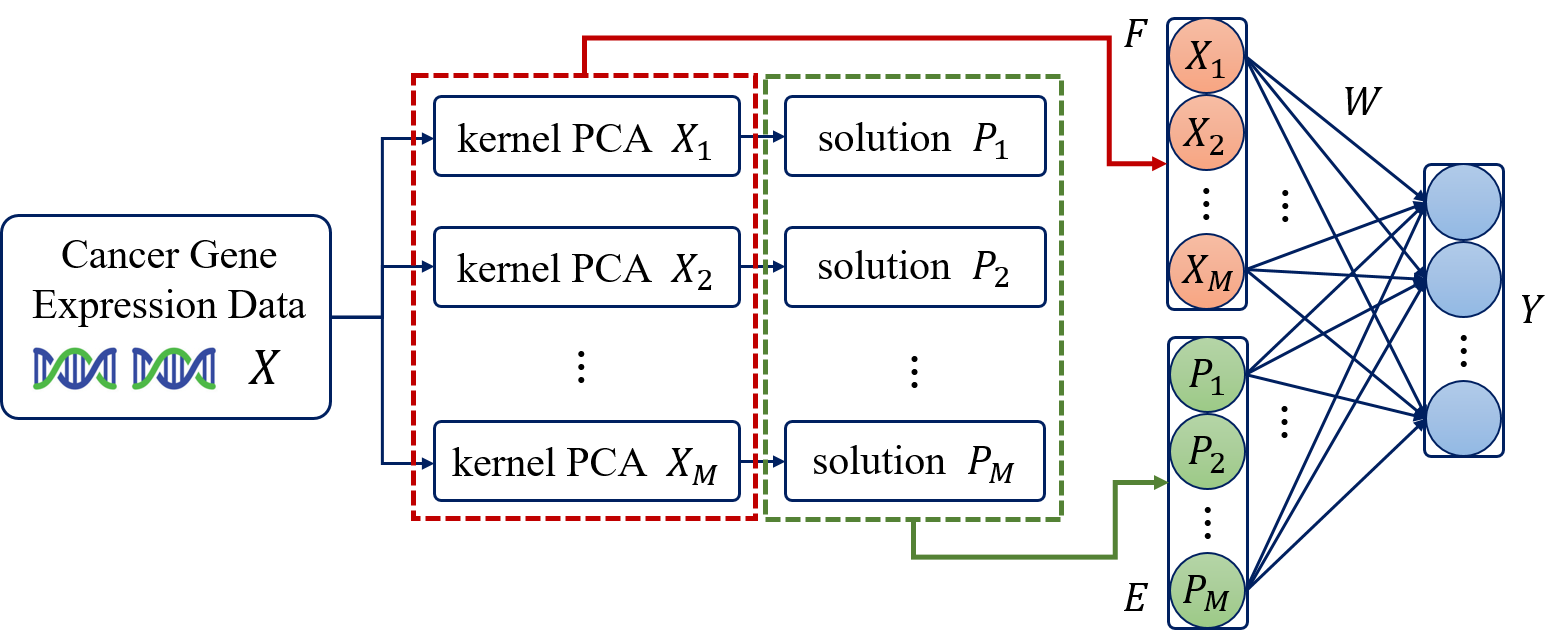
\includegraphics[width=140mm]{./figure/framework.png}\\
	\end{tabular}
	\caption{HCEC的框架图}
	\label{fig_framework}
\end{figure}


\section{算法理论研究}

\subsection{基于核主成分分析的聚类解决方案生成}

具体来说，基因表达数据通常是高维且有噪声的，这很容易干扰底层聚类解决方案的质量。因此，在无监督场景下，我们采用各种核主成分分析（KPCA）方法\cite{Scholkopf1997Kernel}生成多个特征子空间，既避免了噪声干扰，又在一定程度上增加了聚类方案的多样性。KPCA的目标如下：

\begin{equation}\label{eq_KPCA}
	\max{ tr(Q^TZZ^TQ) } ~~ s.t. Q^TQ=I
\end{equation}

其中$Q$为投影矩阵，$Z$为核空间中的数据矩阵。HCEC应用线性核、rbf核和sigmoid核如下：

\begin{equation}
	K_{linear}(x_i,x_j)=x_i\cdot x_j
\end{equation}
\begin{equation}
	K_{rbf}(x_i,x_j)=e^{-\gamma ||x_i-x_j||^2}
\end{equation}
\begin{equation}\label{eq_sigmoid}
	K_{sigmoid}(x_i,x_j)=tanh(\zeta x_i^Tx_j+c)
\end{equation}

对于HCEC生成阶段的第$i$分支，使用选定核的PCA生成低维特征子空间$X_i$，保留数据的$p\in[85\%,98\%]$方差信息。随后，对特征子空间采用K-means，快速生成多个a基聚类解$P_i$。$P_i$可以用二进制分区矩阵表示如下：

\begin{equation}\label{eq_P}
	P_{i(jk)}=\begin{cases}
		1, & if~P_i(x_j)=k \\
		0, & otherwise
	\end{cases}
\end{equation}

其中$P_{i(jk)}$是矩阵$P_i$的$(j,k)$-元素，$P_i(x_j)$表示$x_j$的聚类分配。

\subsection{基于共识宽度学习网络的聚类解决方案集成}
显然，由二元划分矩阵表示的基本聚类解保留了0-1值的样本-聚类关系，这可能导致积分阶段的信息丢失。为了协作来自特征和聚类两个层次的混合信息，HCEC构建了一个共识广泛学习网络（ConBLS）。广义学习系统（BLS） \cite{Chen2017Broad}是一种通过扩展网络的宽度而不是深度来提高学习能力和效率的有效方法。近年来对BLS进行了广泛的研究\cite{Gong2022Research,Zhu2023Distributed}，包括自编码器版本\cite{Yang2021Extracting,yu2023broad}、增量版本\cite{Yang2021Incremental}、堆叠版本\cite{liu2021stacked,Gong2024Cross}、模糊版本\cite{duan2024extreme}、自适应版本\cite{Gong2024CiABL}等。然而，很少有人研究它在无监督学习中的应用。

如图\ref{fig_framework}右半部分所示，ConBLS旨在将所有特征子空间和基本聚类方案组合成一个统一的划分矩阵。具体来说，在CBLS中，隐藏层$H$由特征节点$F$和增强节点$F$组成。传统BLS采用的随机投影方法可能导致性能不稳定，因此，CBLS的特征节点和增强节点分别从$\mathcal{X}$和$\mathcal{P}$进行连接。
\begin{equation}\label{eq_H}
	\begin{aligned}
		& H=[F~|~ E] \\
		s.t.~& F=[X_1~X2~...~X_M] \\
		& E=[P_1~P2~...~P_M]
	\end{aligned}
\end{equation}

ConBLS的输出层为$Y\in \mathbb{R}^{n\times c}$，隐藏层与输出层之间的连接权矩阵为$W\in \mathbb{R}^{l\times c}$，其中$l$和$c$分别为隐藏层的维数和簇的个数。为了协同学习$Y$和$W$， ConBLS的目标函数为：
\begin{equation}
	\min_{Y,W}~L=||Y-HW||^2_F+\alpha ||W||_F^2 + \frac{\beta}{2}\sum_{i=1}^n \sum_{j=1}^n S_{ij}||y_i-y_j||^2_2
\end{equation}

其中$S$为基因表达数据的亲和矩阵，$\alpha$和$\beta$为参数。第一项是重构损失，它学习特征子空间与统一划分矩阵的聚类解之间的映射关系。第二项采用$W$的Frobenius范数对噪声进行惩罚。最后一项保留数据的局部关联。

为清楚起见，目标重新拟订如下：
\begin{equation}
	\min_{Y,W}~\mathcal{L}=||Y-HW||^2_F+\alpha ||W||_F^2 + \beta Tr(Y^TLY)
\end{equation}

其中$L$是拉普拉斯矩阵。由于需要对两个变量矩阵进行优化，所以采用备选优化过程。具体来说，$Y$是由从$\mathcal{P}$中随机选择的二进制分区矩阵初始化的。然后通过固定一个变量并求解另一个变量来迭代更新$W$和$Y$。

\begin{algorithm}[t]
	\caption{面向癌症基因表达数据的混合协同集成聚类算法（HCEC）}
	\label{Alg_1}
	\begin{algorithmic}[1]
		\Require
		\textbf{输入}：癌症基因数据 $X$；基聚类解的数量 $M$；参数 $\alpha$ 和 $\beta$
		\Ensure
		\textbf{输出}：一致性聚类解 $P^*$
		\For{$t=1$ \textbf{to} $M$}
		\State 应用带随机核的主成分分析（PCA），通过式(\ref{eq_KPCA})-(\ref{eq_sigmoid})获得低维表示 $X_t$
		\State 对 $X_t$ 应用K-means算法，获得一个基聚类解
		\State 通过式(\ref{eq_P})计算二值划分矩阵 $P_t$
		\EndFor
		\State 通过式(\ref{eq_H})构建隐层 $H$
		\State 在集合 $\mathcal{P}=\{P_1,P_2,...,P_M\}$ 中用随机划分矩阵初始化 $Y$
		\While{$L$ 未收敛}
		\State 通过式(\ref{eq_W})计算 $W$
		\State 通过式(\ref{eq_Y})计算 $Y$
		\EndWhile
		\State 构建二部图 $\mathcal{G}=\{X,Y\}$
		\State 对 $\mathcal{G}$ 应用TCUT算法，获得一致性聚类解 $P^*$
	\end{algorithmic}
\end{algorithm}


\textbf{（1）固定$Y$，更新$W$}。$L$的最后一项为常数，目标函数为：
\begin{equation}
	\min_{W}~L_W=||Y-HW||^2_F+\alpha ||W||_F^2
\end{equation}

为了最小化$L_W$，我们将$W$的偏导数设为0，如下所示：

\begin{equation}\label{eq_LW}
	\frac{\partial L_W}{\partial W}=||Y-HW||^2_F+\alpha ||W||_F^2=0
\end{equation}

当$n>l$和式（\ref{eq_LW}）具有近似解时，$H$为满秩。
\begin{equation}
	W=(\alpha I+H^TH)^{-1}H^TY
\end{equation}

另一方面，当$n\leq l$时，式（\ref{eq_LW}）有无穷个待定解。为了得到唯一解，$W$受到$W=HG$的约束，其中$G\in \mathbb{R}^{n\times n}$和$(AA^T)^{-1}$乘以方程（\ref{eq_LW}）的两边，以计算备选解。
\begin{equation}
	W=H^T(\alpha I+HH^T)^{-1}Y
\end{equation}

综上，$W$的更新公式如下：
\begin{equation}\label{eq_W}
	W=\begin{cases}
		(\alpha I+H^TH)^{-1}H^TY, & n>l \\
		H^T(\alpha I+HH^T)^{-1}Y, & otherwise
	\end{cases}
\end{equation}


\textbf{（2）固定$W$，更新$Y$}。第二项为常数，目标函数变为：
\begin{equation}
	\min_{Y}~L_Y=||Y-HW||^2_F+\beta Tr(Y^TLY)
\end{equation}

通过设置$L_Y$的偏导数为0，计算$Y$的解如下：
\begin{equation}\label{eq_Y}
	Y=(I+\beta L)^{-1}HW
\end{equation}

求解ConBLS后，得到统一的划分矩阵$Y$，反映了样本与聚类之间的协关联关系。因此，通过$\mathcal{G}=\{V,Y\}$构造了一个非直接二部图。$V$是同时包含样本和集群的图节点。样本节点和簇节点之间的链接权值由$Y$提供。样本节点或集群节点之间没有链接。在二部图的基础上，应用TCUT \cite{Li2012Segmentation}\cite{Huang2017Locally}将图划分为$c$个不相交子图。在一致聚类解中，同一子图中的样本节点组成一个聚类。

\section{算法代码实现}

\chapter{实验}\label{chapter_exp}

\section{数据集和实验设置}
在实验中，如表\ref{tab_dataset}所示，采用6个癌症基因表达数据集\cite{UCI2013dataset}来测试所提出方法的性能。可以看出，基因表达数据通常具有大量的特征，并且可能包含噪声特征，这对聚类来说是一个挑战。

\begin{table}[tbh]
	\caption{数据集概述}\label{tab_dataset}
	\centering
	\begin{tabular} {l l|c c c}
		\hline
		$\#$ & Dataset & $n$ & $d$ & $k$ \\
		\hline
		D1 & Alizadeh-2000-v3 & 62 & 2093 & 4 \\
		D2 & Armstrong-2002-v2 & 72 & 2194 & 3 \\
		D3 & Bredel-2005 & 50 & 1739 & 3 \\
		D4 & Lapointe-2004-v1 & 69 & 1625 & 3 \\
		D5 & Alizadeh-2000-v3  & 62 & 4026 & 4 \\
		D6 & Su-2001 & 174 & 1571 & 10 \\
		\hline
	\end{tabular}
\end{table}

为了全面衡量聚类的性能，我们采用归一化互信息\cite{strehl2002cluster}和调整后的兰德指数\cite{Hubert2003Comparing}指标，分别以$NMI$和$ARI$命名。
\begin{equation}
	\begin{aligned}
		& NMI(P^*,P^g)=  \frac{2\sum_{i=1}^{k}\sum_{j=1}^{k}\frac{|C^*_i\cap C^g_j|}{n}log\frac{n|C^*_i\cap C^g_j|}{|C^*_i||C^g_j|}}{-\sum_{i=1}^{k}\frac{|C^*_i|}{n}log\frac{|C^*_i|}{n}-\sum_{j=1}^{k}\frac{|C^g_j|}{n}log\frac{|C^g_j|}{n}}
	\end{aligned}
	\label{Eq33}
\end{equation}
\begin{equation}\label{eq_ARI}
	\begin{aligned}
		& ARI(P^*,P^g)= \frac{\sum_{i=1}^{k}\sum_{j=1}^{k}\binom{|C^*_i\cap C^g_j|}{2}-\Omega_3}{(\Omega_1+\Omega_2)/2-\Omega_3} \\
		& \Omega_1=\sum_{i=1}^{k}\binom{|C^*_i|}{2},~\Omega_2=\sum_{j=1}^{k}\binom{|C^g_j|}{2},~\Omega_3=\frac{2\Omega_1\Omega_2}{n(n-1)}
	\end{aligned}
\end{equation}

其中$P^*$和$P^g$分别表示共识解和基真解，$C_i$为对应的聚类。越高的$NMI\in[0,1]$和$ARI\in[-1,1]$表示越好的聚类解决方案。

\section{参数分析}

HCEC涉及两个参数$\alpha$和$\beta$，分别用于控制惩罚项和亲和结构约束。为了验证这些参数对模型的影响，我们在$[1e^{-3},1e^{-2},1e^{-1},1,1e^{1},1e^{2},1e^{3}]$中进行了网格搜索，并绘制了3D热图，以显示不同参数组合下HCEC的聚类性能。在4个数据集上的实验结果如图\ref{fig_param}所示，从图中可以看出，HCEC在$\beta \in [1e^{-3},1e^{-1}]$的一定范围内表现较好，并且HCEC对alpha的选择并不是特别敏感。一般来说，HCEC的参数选择相对宽松和灵活，可以采用聚类有效性指标进行指导。

\begin{figure}[h]
	\centering
	\begin{tabular}{ccc}
		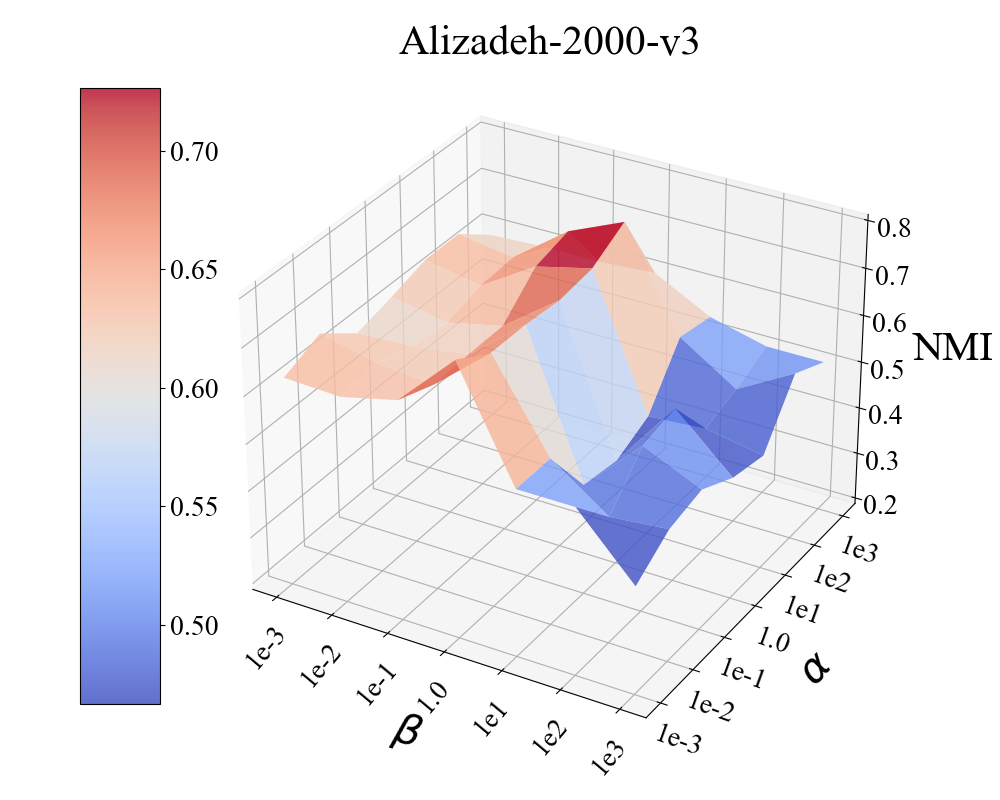
\includegraphics[width=0.45\textwidth]{./figure/param_d1.png}&
		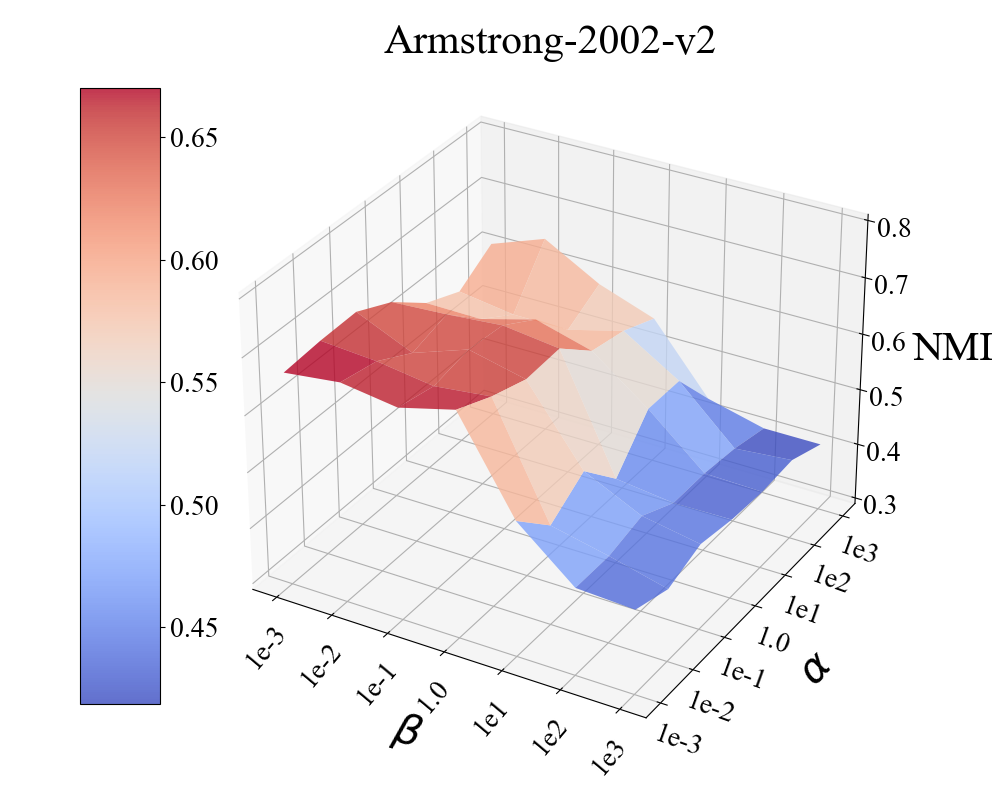
\includegraphics[width=0.45\textwidth]{./figure/param_d2.png}
		\\
		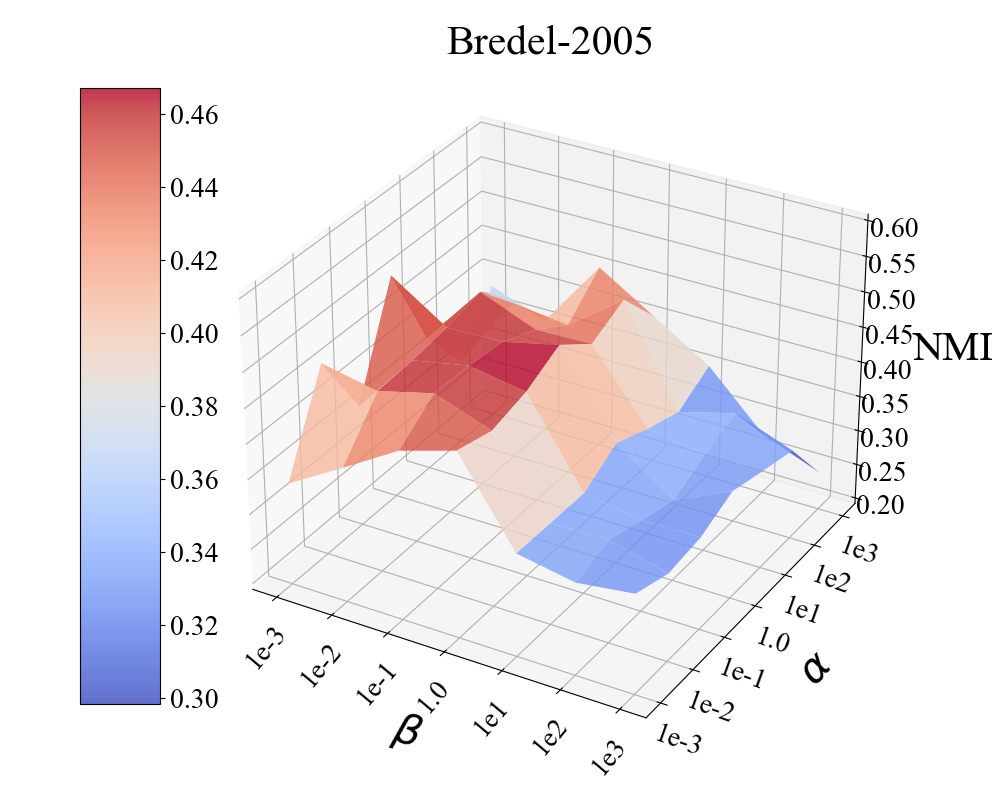
\includegraphics[width=0.45\textwidth]{./figure/param_d3.png}&
		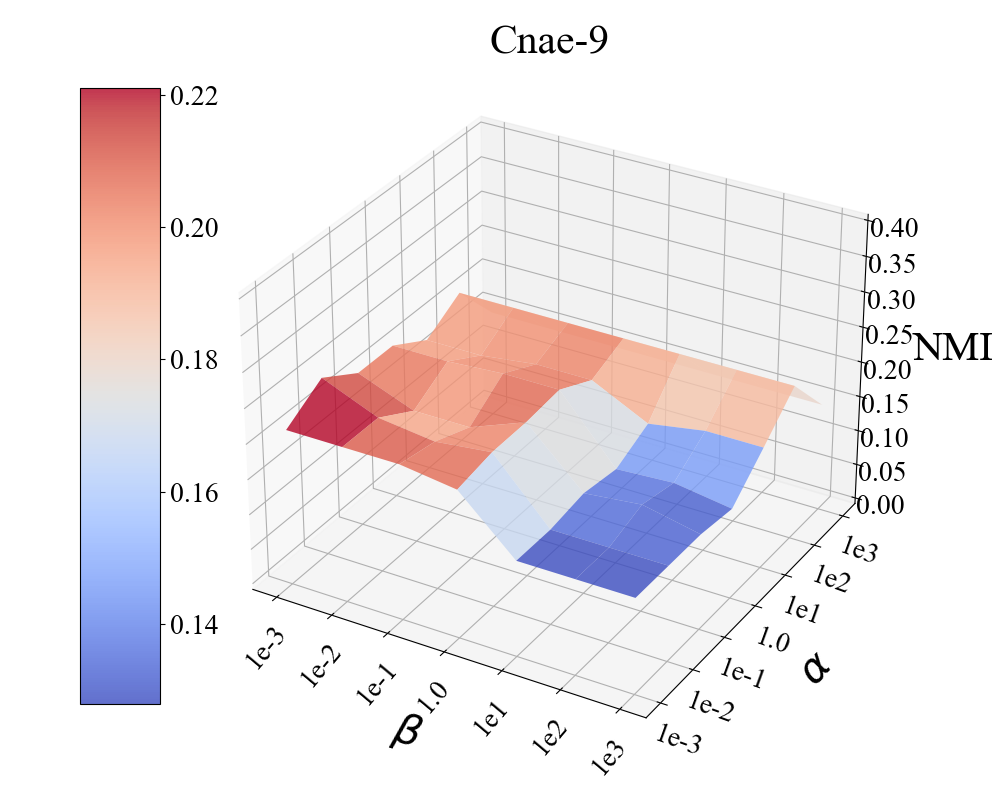
\includegraphics[width=0.45\textwidth]{./figure/param_d4.png}
	\end{tabular}
	\caption{$NMI$测量下参数$\alpha$和$\beta$的影响}
	\label{fig_param}
\end{figure}


\section{对比实验与分析}
为了验证算法，我们将HCEC与聚类算法进行了比较，包括2种单模型聚类算法和6种集成聚类算法（\textit{即}CSPA \cite{strehl2002cluster}、EAC \cite{Fred2005Combining}、LWEC \cite{Huang2017Locally}、ECPCS \cite{Huang2021Enhanced}、SORTHMC \cite{Yu2022Clustering}和BoostAEC \cite{Shi2023Adaptive}）。对于所有比较方法，基本聚类解决方案的数量设置为20。此外，这些方法的参数设置都是根据其原始论文中的建议进行的。这些算法在$NMI$和$ARI$下的聚类性能分别如表\ref{tab_compare_nmi}和表\ref{tab_compare_ari}所示，最好的结果以粗体显示。

通过算法比较可以看出，传统的单模型聚类方法（K-means和谱聚类）表现最差，特别是谱聚类在处理高维噪声基因数据时表现最差。相比之下，集成聚类方法取得了显著的性能改进。通过整合多视角投影子空间和簇结构，HECE在$NMI$和$ARI$指标中分别获得了1.3333和1.1667的平均排名。

\begin{table*}[t]
	\caption{基于$NMI$测量下的不同聚类方法的比较结果}
	\label{tab_compare_nmi}
	\renewcommand{\arraystretch}{1.2}
	\centering
	\resizebox{\textwidth}{!}{
		\begin{tabular}{c|ccccccccc}
			\hline
			Dataset & K-means & SC & CSPA & EAC & LWEC & ECPCS & SORTHMC & BoostAEC & HCEC \\
			\hline
			D1 & 0.4258 & 0.1241 & 0.5262 & 0.5085 & 0.5366 & 0.5904 & 0.5428 & 0.6365 & \textbf{0.7212} \\
			D2 & 0.5348 & 0.0473 & 0.5662 & 0.5672 & 0.6194 & 0.6311 & 0.6588 & 0.5920 & \textbf{0.6629} \\
			D3 & 0.3311 & 0.0709 & 0.2634 & 0.3184 & 0.3698 & 0.3447 & 0.3691 & 0.4054 & \textbf{0.4624} \\
			D4 & 0.1187 & 0.1260 & 0.1417 & 0.1733 & 0.1837 & 0.1899 & 0.2022 & \textbf{0.2193} & 0.2117 \\
			D5 & 0.5242 & 0.0357 & 0.5097 & 0.5166 & 0.5671 & 0.5954 & 0.5661 & 0.6332 & \textbf{0.7734} \\
			D6 & 0.5900 & 0.2690 & 0.7034 & 0.6820 & 0.7084 & 0.7155 & \textbf{0.7413} & 0.7017 & 0.7305 \\
			\hline
			AvgRanking & 7.5000 & 8.8333 & 6.8333 & 6.6667 & 4.1667 & 3.5000 & 3.1667 & 3.0000 & \textbf{1.3333} \\
			\hline
		\end{tabular}
	}
\end{table*}


\begin{table*}[t]
	\caption{基于$ARI$测量下的不同聚类方法的比较结果}
	\label{tab_compare_ari}
	\renewcommand{\arraystretch}{1.2}
	\centering
	\resizebox{\textwidth}{!}{
		\begin{tabular}{c|ccccccccc}
			\hline
			Dataset & K-means & SC & CSPA & EAC & LWEC & ECPCS & SORTHMC & BoostAEC & HCEC \\
			\hline
			D1 & 0.2684 & 0.0227 & 0.3504 & 0.3308 & 0.3448 & 0.3955 & 0.3684 & 0.4403 & \textbf{0.5154} \\
			D2 & 0.4872 & 0.0019 & 0.5297 & 0.5316 & 0.5730 & 0.6045 & 0.5992 & 0.5395 & \textbf{0.6107} \\
			D3 & 0.3044 & 0.0228 & 0.2004 & 0.2637 & 0.3240 & 0.2768 & 0.2701 & 0.3537 & \textbf{0.5194} \\
			D4 & 0.1007 & 0.0691 & 0.1429 & 0.1646 & 0.1875 & 0.1830 & 0.1841 & 0.1934 & \textbf{0.1984} \\
			D5 & 0.3764 & 0.0049 & 0.3784 & 0.3294 & 0.3860 & 0.4123 & 0.3780 & 0.4445 & \textbf{0.5334} \\
			D6 & 0.3965 & 0.0323 & 0.5854 & 0.5629 & 0.5839 & 0.6075 & \textbf{0.6608} & 0.6001 & 0.6578 \\
			\hline
			AvgRanking & 7.1667 & 9.0000 & 6.1667 & 6.8333 & 4.3333 & 3.5000 & 4.0000 & 2.8333 & \textbf{1.1667} \\
			\hline
		\end{tabular}
	}
\end{table*}


\section{消融实验与分析}
为了验证HCEC的每个组成部分，我们进一步进行了消融分析。具体来说，我们比较了以下几种方法：1)HCEC-RS：在生成阶段，利用随机子空间技术代替核主成分分析；2) HCEC-CSPA：在整合阶段，用CSPA的常规共识方法代替ConBLS \cite{strehl2002cluster}；3) HCEC：提出的用于癌症基因表达数据的混合协同集成聚类。通过$NMI$和$ARI$测量的消融实验分析如图所示。\ref{fig_ablation_nmi} - \ref{fig_ablation_ari}。可以看出，HCEC比HCEC- rs和HCEC- cspa表现出明显的性能优势，表明核化PCA可以减少噪声特征的影响，ConBLS可以有效地整合特征层和聚类层的混合知识，从而提高聚类性能。

\begin{figure}[tbh]
	\centering
	\begin{tabular}{p{14cm}}
		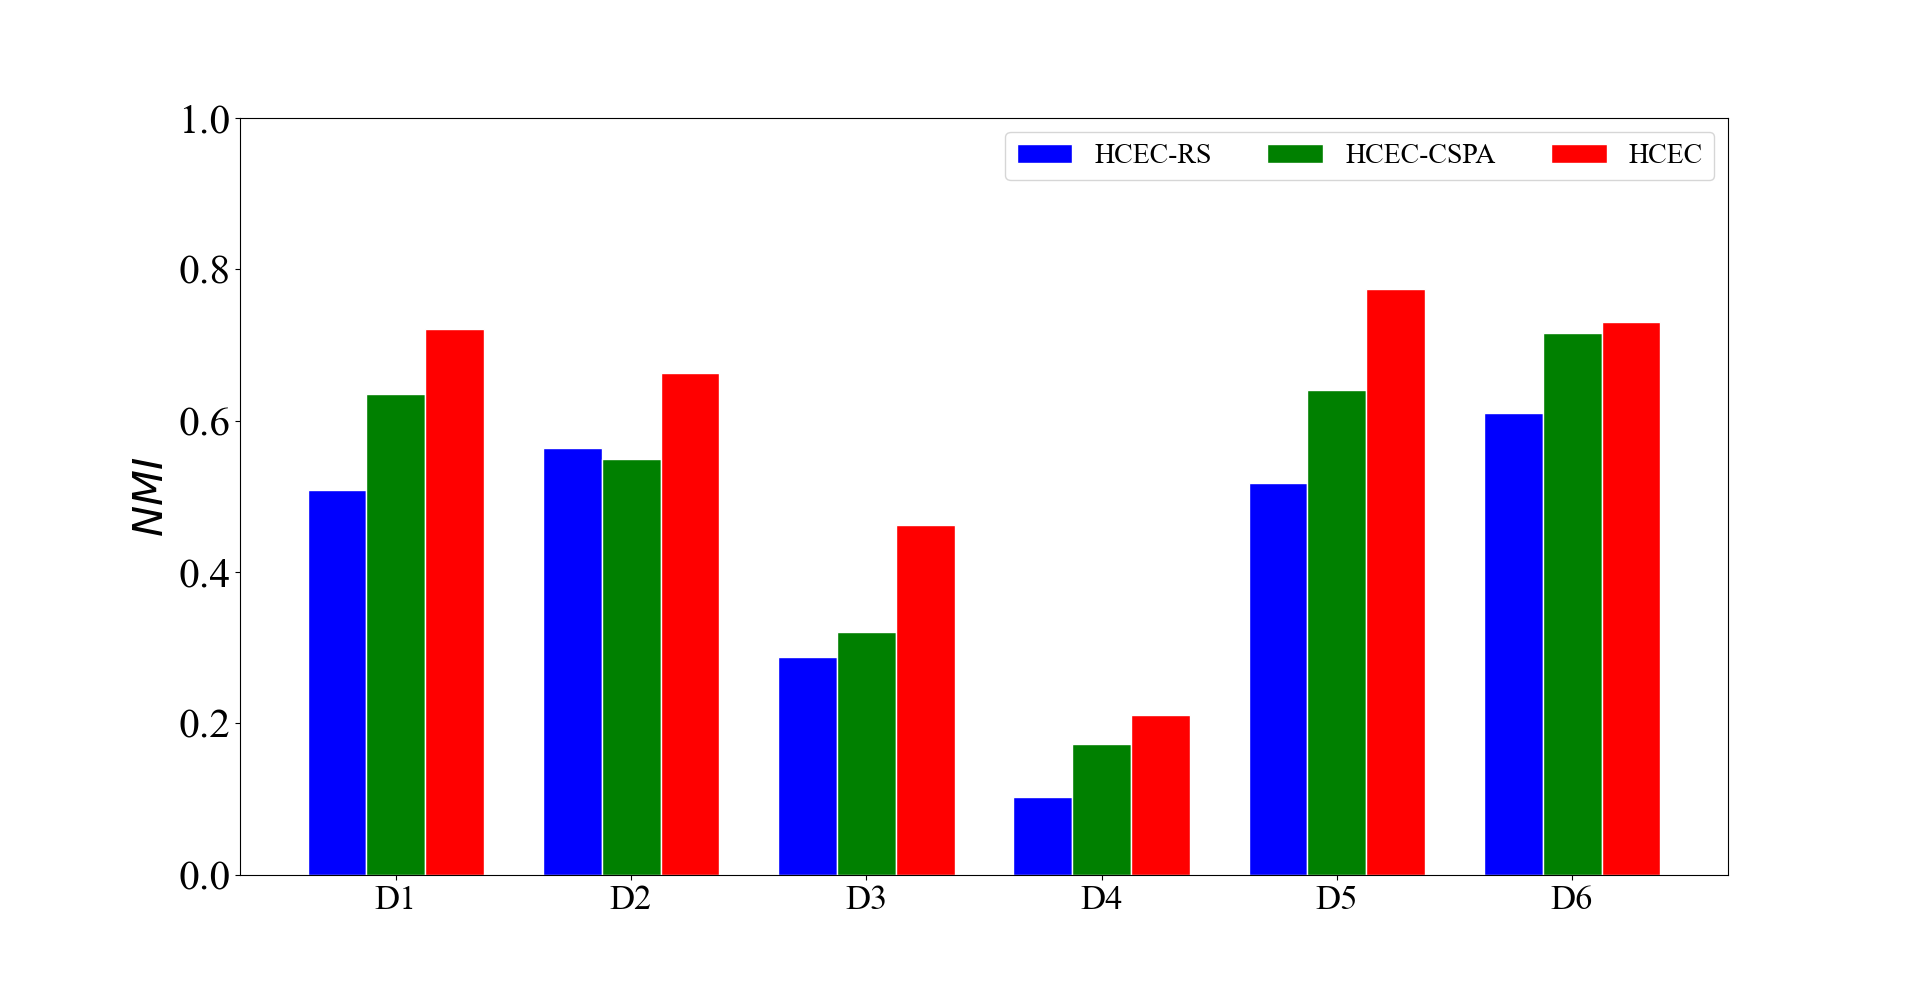
\includegraphics[width=140mm]{./figure/ablation_nmi.png}\\
	\end{tabular}
	\caption{基于$NMI$测量的消融实验结果柱状图}
	\label{fig_ablation_nmi}
\end{figure}

\begin{figure}[tbh]
	\centering
	\begin{tabular}{p{14cm}}
		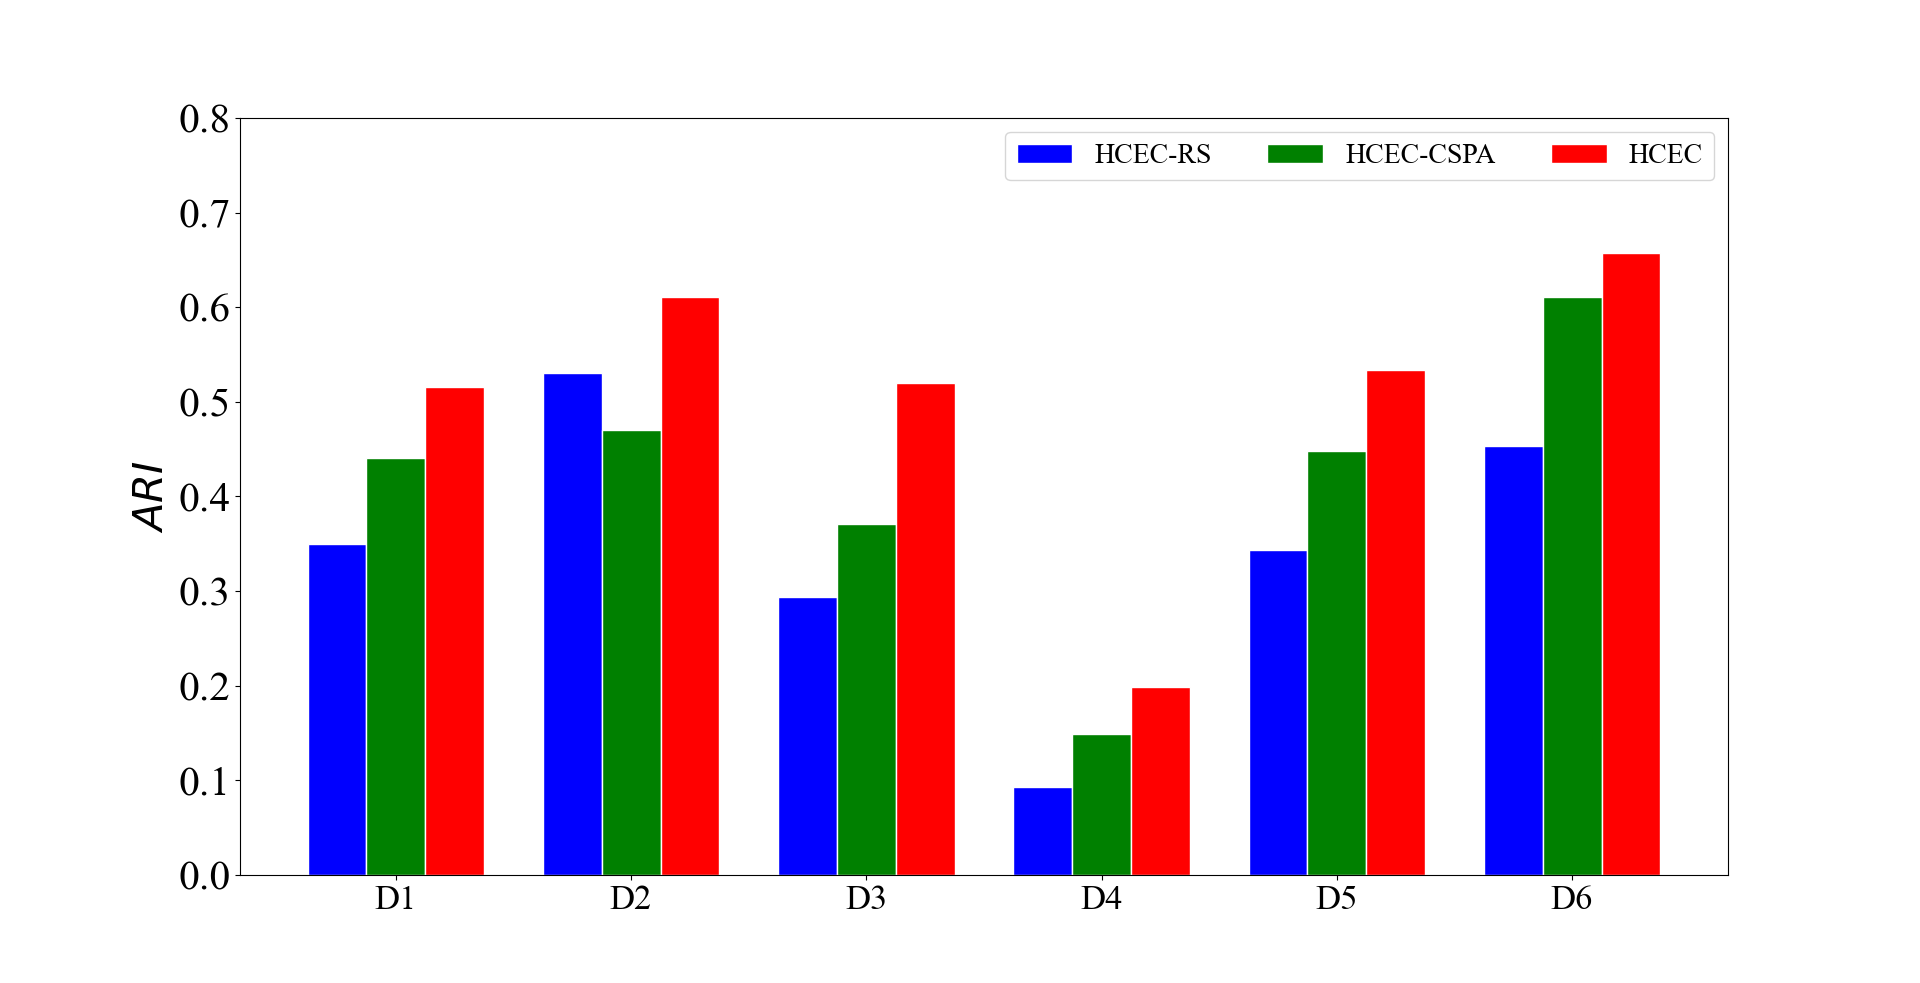
\includegraphics[width=140mm]{./figure/ablation_ari.png}\\
	\end{tabular}
	\caption{基于$ARI$测量的消融实验结果柱状图}
	\label{fig_ablation_ari}
\end{figure}


\chapter{总结与展望}
本文通过设计混合协作集成聚类框架来解决癌症基因表达数据的挑战。采用核主成分分析和多聚类技术，获得了基因表达谱的多视角特征。随后，我们构建共识广义学习网络，有效整合包含多特征子空间和聚类结构的混合信息，从而提高共识解的性能。通过参数分析、对比实验和对多个真实世界癌症基因数据集的消融研究，证明了HCEC的有效性。在未来的工作中，我们将进一步设计一个优化过程来学习特征子空间和聚类结构，以获得更鲁棒和准确的聚类性能，并将其应用于各种医疗保健任务。

全文的内容总结，

（1）全文的内容总结，

（2）全文的内容总结，

（3）全文的内容总结，


\backmatter

%%%%%%%%%%%%%%%%%%%%%%%%%%%%%参考文献%%%%%%%%%%%%%%%%%%%%%%%%%%%%%%

\bibliographystyle{hquthesis}%参考文献格式文件，hquthesis.bst
\bibliography{reference}%收录参考文献的bib文件，reference.bib，如需要换成


\chapterx{致\ 谢}

论文致谢部分，论文致谢部分，论文致谢部分，论文致谢部分，论文致谢部分，论文致谢部分，论文致谢部分，论文致谢部分，论文致谢部分，论文致谢部分，论文致谢部分，论文致谢部分，论文致谢部分，论文致谢部分，论文致谢部分，论文致谢部分，论文致谢部分，论文致谢部分，论文致谢部分，论文致谢部分，论文致谢部分，论文致谢部分，论文致谢部分，论文致谢部分，论文致谢部分，论文致谢部分，论文致谢部分，论文致谢部分，论文致谢部分，论文致谢部分，论文致谢部分，论文致谢部分，论文致谢部分，论文致谢部分，论文致谢部分，论文致谢部分，论文致谢部分，论文致谢部分，论文致谢部分，论文致谢部分，论文致谢部分，论文致谢部分，论文致谢部分，论文致谢部分，论文致谢部分，论文致谢部分，论文致谢部分，论文致谢部分，论文致谢部分，论文致谢部分，论文致谢部分，论文致谢部分，论文致谢部分，论文致谢部分，论文致谢部分，论文致谢部分，论文致谢部分，论文致谢部分，论文致谢部分，论文致谢部分，论文致谢部分，论文致谢部分，论文致谢部分，论文致谢部分，论文致谢部分，论文致谢部分，论文致谢部分，论文致谢部分，论文致谢部分，论文致谢部分，论文致谢部分，论文致谢部分，论文致谢部分，论文致谢部分，论文致谢部分，论文致谢部分，论文致谢部分，论文致谢部分，论文致谢部分，论文致谢部分，论文致谢部分，论文致谢部分，论文致谢部分，论文致谢部分，论文致谢部分，

~\\

\begin{minipage}[t]{0.945\textwidth}%
\begin{flushright}
李毅\\
%\today\\
2026年4月21日于华侨大学%可注释删除
\par\end{flushright}
\end{minipage}

\appendix{附\ 录}
%重新设置表、图、公式的序号和格式，否则接着前面的继续编号       added by YYS
\setcounter{table}{0}
\setcounter{figure}{0}
\setcounter{equation}{0}
\renewcommand{\theequation}{\textbf{A}-\arabic{equation}}%格式为A开头加序号，如A-1，A-2
\renewcommand{\thetable}{\textbf{A}-\arabic{table}}%格式为A开头加序号，如A-1，A-2
\renewcommand{\thefigure}{\textbf{A}-\arabic{figure}}%格式为A开头加序号，如A-1，A-2
\section{在读期间获得的科研成果}

(1) 张三获得2019年xxxxx科创奖，排名第一

(2) Zhang S, Li S, Wang W, et al. How to Love Huaqiao University [J]. IEEE Transaction on Image Processing, 2021, 34(7): 1000-1002

(3) 张三，李四，王五. 一种建设好工学院的神奇装置.发明专利（或者实用发明专利），专利号（或者申请号）：xxxx

(4) 张三，李四，王五. 一种自动想念华侨大学的算法. 软件著作权，登记号：xxxx

\section{关于xxx的代码实现}


\section{关于xxx的数学推导}

%

\end{document}
